 \documentclass[a4paper,12pt]{article}
 
 \usepackage{amsmath}
 \usepackage{mathtools}
 \usepackage{amssymb}
 \usepackage{graphicx}
 \usepackage{hyperref}
 \usepackage{url}
 \usepackage[authoryear]{natbib}  
 % \usepackage{csquotes} 
 %\usepackage{color}
 \usepackage[dvipsnames]{xcolor}
 
 %Comandi Utili
 \newcommand{\red}[1]{\textcolor{red}{ #1}}
 \newcommand{\tonde}[1]{\left(#1\right)}
 \newcommand{\pt}[1]{\left(#1\right)}
 \newcommand{\pq}[1]{\left[#1\right]}
 \newcommand{\pg}[1]{\left\lbrace#1\right\rbrace}
 \newcommand{\quadre}[1]{\left[#1\right]}
 \newcommand{\abs}[1]{\left\vert #1 \right\vert}
 \newcommand{\graffe}[1]{\left\{#1\right\}}
 \newcommand{\var}[1]{\text{Var}\left(#1\right)}
 \newcommand{\ex}[1]{\text{E}\left[#1\right]}
 \newcommand{\E}[1]{\mathbb{E}\left[#1\right]}
 
 \newcommand{\be}{\begin{equation}}
 \newcommand{\ee}{\end{equation}}
 \newcommand{\ba}{\begin{eqnarray}}
 \newcommand{\ea}{\end{eqnarray}}
 \newcommand{\y}{{\mathbf{y}}}
 \newcommand{\Y}{{\mathbf{Y}}}
 \newcommand{\Yt}{{\mathbf{Y}^{\tonde{t}}}}
 \newcommand{\Ytm}{{\mathbf{Y}^{\tonde{t-1}}}}
 \newcommand{\Yijt}{{Y_{ij}^{\tonde{t}}}}
 \newcommand{\Yij}{{Y_{ij}}}
 \newcommand{\Yijtm}{{Y_{ij}^{\tonde{t - 1}}}}
 \newcommand{\x}{{\mathbf{x}}}
 \newcommand{\X}{{\mathbf{X}}}
 \newcommand{\Xt}{{\mathbf{X}^{\tonde{t}}}}
 \newcommand{\Xtm}{{\mathbf{X}^{\tonde{t-1}}}}
 \newcommand{\Xijt}{{X_{ij}^{\tonde{t}}}}
 \newcommand{\Xij}{{X_{ij}}}
 \newcommand{\Xijtm}{{X_{ij}^{\tonde{t - 1}}}}
 \newcommand{\A}{{\mathbf{A}}}
 \newcommand{\At}{{\mathbf{A}^{\tonde{t}}}}
 \newcommand{\Atm}{{\mathbf{A}^{\tonde{t-1}}}}
 \newcommand{\Aijt}{{A_{ij}^{\tonde{t}}}}
 \newcommand{\Aijtm}{{A_{ij}^{\tonde{t - 1}}}}
 \newcommand{\score}[1]{\left. \frac{\partial \log{l}}{\partial f}\right|_{\tonde{ #1 }} }
 \newcommand{\etmmm}{^{\tonde{t-3}}}
 \newcommand{\etmm}{^{\tonde{t-2}}}
 \newcommand{\etm}{^{\tonde{t-1}}}
 \newcommand{\et}{^{\tonde{t}}}
 \newcommand{\uij}{_{ij}}
 \newcommand{\e}[1]{^{\tonde{#1}}}
 \newcommand{\etprime}{^{\tonde{t}\prime}}
 \newcommand{\etp}{^{\tonde{t+1}}}
 \newcommand{\bobeta}{\boldsymbol{\beta}}
 \newcommand{\binpar}{\theta}
 \newcommand{\bobinpar}{\boldsymbol{\binpar}}
 \newcommand{\ibinpar}{{\overleftarrow{\binpar}}}
 \newcommand{\obinpar}{{\overrightarrow{\binpar}}}
 \newcommand{\wpar}{\varphi}
 \newcommand{\iwpar}{{\overleftarrow{\wpar}}}
 \newcommand{\owpar}{{\overrightarrow{\wpar}}}
 \newcommand{\wparvar}{\eta}
 \newcommand{\iwparvar}{{\overleftarrow{\wparvar}}}
 \newcommand{\owparvar}{{\overrightarrow{\wparvar}}}
 \newcommand{\onpar}[1]{ {\overrightarrow{#1}}}
 \newcommand{\inpar}[1]{ {\overleftarrow{#1}}}
 \newcommand{\wparexp}{\delta}
 \newcommand{\iwparexp}{{\overleftarrow{\wparexp}}}
 \newcommand{\owparexp}{{\overrightarrow{\wparexp}}}
 \newcommand{\istr}{{\overleftarrow{S}}}
 \newcommand{\ostr}{{\overrightarrow{S}}}
 \newcommand{\vectwoc}[2]{ \left( \begin{array}{c} #1 \\ \\ #2  \end{array}  \right)    }
 
 
 
 \newcommand{\alsum}{ \tonde{\lambda_n + \eta_k}}
 \newcommand{\besum}{ \tonde{\rho_n + \delta_k}}
 \newcommand{\deno}{1 + e^{\quadre{\besum - e^{-\alsum}}} - e^{- e^{-\alsum}}}
 \newcommand*\rotnine{\rotatebox{90}}
 \newcommand*\rotfour{\rotatebox{45}}
 \newcommand*\OK{\ding{51}}
 
 \DeclareMathOperator{\prob}{\Wathrm{Prob}}
 \DeclareMathOperator{\prior}{\Wathrm{Prior}}
 \newcommand{\argmax}[1]{\underset{#1}{\operatorname{arg}\,\operatorname{max}}\;}
 \newcommand{\argmin}[1]{\underset{#1}{\operatorname{arg}\,\operatorname{min}}\;}
 
 %Options to set a layout of the page
 %--------------
 \addtolength{\hoffset}{-3cm}
 \addtolength{\textwidth}{4cm}
 \addtolength{\textheight}{5cm}
 \addtolength{\voffset}{-4cm}
 
 
\title{Zero Augmented Generalized Linear Models with Score Driven Parameters for Sparse Weighted Dynamical Networks \\( With Applications to Systemic Risk Forecasting ?)}
\author{Domenico Di Gangi}
\begin{document}
\maketitle
\section*{Domande aperte}
\begin{itemize}
	\item La motivazione del paper sarebbe : 
		\begin{itemize}
			\item Contribuire alla scarsa letteratura su modelli dinamici per reti sparse e pesate, unendo networks ZA and score driven models.
			\item Affronta il problema della high dimensionality delle possibili strutture di dipendenza temporale con combinazione fitnesses (parametri node specific) + SD 
			\item Permette di disaccoppiare la propensione alle connessioni intrinseca di ogni nodo (fitnesses) dal contributo dovuto a un qualunque regressore. In un certo senso, \'e simile al paper sul DAR-Fitness per la persistenza. Quindi le fitnesses (binarie o pesate), quando usate congiuntamente con i regressori, potrebbe essere proposte come propensione ad avere connessioni (o connessioni di peso) che non sono spiegate dai regressori
			\item Usando a validazione in sample e out of sample per model selection, consente di rispondere alla domanda: il regressore X \'e importante per la dinamica della rete? Quali sono le fitnesses al netto dell'effetto del regressore?
		\end{itemize}

	
	
	\item Ha senso discutere anche il forecast della rete? i.e. combinazione di forecast binario e pesato? Forse si potrebbe fare per mostrare una possibile applicazione a financial stability.
	
	
	
	\item commenti sulla struttura? 
	\begin{itemize}
		\item non sono sicuro se aggiungere una sezione solo per i modelli score driven. 
		\item presento prima dinamica per parametri associati ai pesi e poi per la versione binaria. controintuitivo? Vorrei sottolineare che la dinamica SD per i pesi \'e la parte principale del lavoro. oltre a essere indipendente da quella dei links e quindi applicabile con altri modelli binari		
	\end{itemize}
\end{itemize}
\newpage

\section*{Paper Structure}
\begin{enumerate}
\item Introduction: we intend to model dynamical sparse weighted networks. 

The main challenges are: sparcity and high dimensionality.

Review of existing literature. 

We use Zero Augmentation and Score Driven version of meaningful static models, adding the possibility of dependency on external variables.

Paper outline.
\item Methods:  Zero augmentation in general to address sparcity 

  Score Driven version of  static Zero Augmented model with one parameter per node to address high dimensionality. Our approach addresses the challenges mentioned and is flexible enough to allow for additional regressors (separately in links' presence and links' weights). 
  
  Possibility to change the distribution of the weights

Description of models and numerical tests independent of the sequence of binary probabilities. Combination with a similar approach for the binary network (SD-beta model with regressors) for a completely score driven dynamics
\item Applications:  application to WTN and eMid that highlights the possibility of using standard model selection techniques (AIC, BIC, other ideas?) to compare different models. Both SD vs sequence of single snapshots, and different regressors in determining links' presence and weights for different weights distributions. 

Description of forecasting approach and out of sample validation and comparison of different models. 

Final application of forecasting debt rank in eMid?

\end{enumerate}

\newpage
\section{Introduction}
MOTIVATION FOR WEIGHTED NETWORKS\\

NEED FOR SPARCITY\\

We focus on models for  \textbf{Dynamical Sparse Weighted Networks} described by sequences of matrices of positive real numbers $\pg{\Yijt}_{t=1}^{T}$.\\

MOTIVATION FOR DYNAMICS, DISTINCTION BETWEEN GROWTH AND "STATIONARY" (FIXED NUMBER OF NODES) MODELS\\

CHALLENGES AND LITERATURE REVIEW: \\
The goal is to model $P\pt{\Yijt\vert \Y\e{t-1},\dots \Y\e{1}}$. Even if we consider dependencies at one lag, the problem is extremely high dimensional. To cope with the issue of dimensionality, different approaches have been considered in the literature:
\begin{itemize}
	\item  Driven by system specific insights, the researcher selects a set of network statistics $G_i\pt{\Y}$ and estimates the dependency of links at time $t$ on $G\pt{\Ytm}$. \cite{giraitis2016estimating}, for example, estimate a Tobit model with few regressors, for each link. Moreover they use a local-likelihood method to estimate time varying coefficients of the regression. 
	\item Latent space models, where a set of parameters is associated to each node and an exogenous time evolution is assumed for those parameters, e.g.  \cite{sewell2015latent} define a latent space Tobit 
	\item Models that allow each one of the matrix elements $\Yijt$ to depend on each of the $\Yij\etm$ have also been considered in the literature:
	\begin{enumerate}
		\item \cite{billio2018bayesian} Estimate a tensor regression (very similar to a VAR on $vec(\Y)$), with rank restrictions on the (huge) matrix of model's parameters . (Not clear how they take sparsity into account)
		\item \cite{doi:10.1080/02664763.2017.1357684} Consider a penalized logistic auto-regression model for binary networks (basically a logistic regression for each link, using all lagged matrix elements, and also products, with a lasso penalization). The same approach can in principle be extended to sparse weighted networks, and in the ZA framework.
	\end{enumerate}
\end{itemize}

REVIEW OF SCORE DRIVEN MODELS\\

In order to review the score-driven models as introduced by~\cite{creal2013generalized} and~\cite{harvey_2013}, let us consider a sequence of observations $\graffe{y\et}_{t=1}^T$, where each $y\et \in\mathbb{R}^M$,  and a conditional probability density $P\tonde{y\et\vert f\et}$, that depends on a vector of time-varying parameters $f\et \in \mathbb{R}^K$. Defining the score as $\nabla\et = \frac{\partial \log{P\tonde{y\et\vert f\et}}}{\partial f\etprime}$, a score-driven model assumes that the time evolution of $f\et$ is ruled by the recursive relation
\be  \label{eq:gasupdaterule}
f\etp = w +\boldsymbol{\beta} f\et + \boldsymbol{\sigma} \boldsymbol{S\et} \nabla\et , \\
\ee 
where $w$, $\boldsymbol{\sigma}$ and $\boldsymbol{\beta}$ are static parameters, $w$ being a $K$ dimensional vector and $\boldsymbol{\sigma}$ and $\boldsymbol{\beta}$  $K\times K$ matrices.  $\boldsymbol{S\et}$ is a $K\times K$ scaling matrix, that is often chosen to be the inverse of the square root of the Fisher information matrix associated with $P\tonde{y\et\vert f\et}$, i.e. $\boldsymbol{S\et} = \mathbb{E}\quadre{\frac{\partial \log{P\tonde{y\et\vert f\et}}}{\partial f\etprime} \frac{\partial \log{P\tonde{y\et\vert f\et}}}{\partial f\etprime}^\prime }^{-\frac{1}{2}}$. However, this is not the only possible specification and different choices for the scaling are discussed in~\cite{creal2013generalized}.


OUR APPROACH\\

\begin{itemize}
	\item \textbf{We propose} to  start from a static model (in principle one that fits well the cross sectional data ) and define its dynamical version using the SD approach. Applying this to the ZA-Gamma model results in the \textbf{Zero Augmented Score Driven (Gamma?) Network Model ZA-SD-Nets (or maybe weighted random graphs ?ZA-SD-WRG )} 
	
	\item We consider  Zero Augmented distributions to define a framework for a flexible description of \textbf{Sparse Weighted Networks}, already at the static level:
	\ba\label{eq:ZeroAugWeightedNets}
	&P\tonde{\Yij  = y} =  \left\lbrace\begin{array}{ll} 	  \pt{1-p\uij} \quad &for \quad y=0 \\
		\nonumber\\
		p\uij  \; g \tonde{y\vert \mu\uij, \sigma\uij } \quad &for \quad y>0 \end{array}\right. ,\\
	\ea
	where $0<p\uij<1$ and $g\pt{y} $ is the density for a positive continuous random variable, with link specific parameters $\mu\uij$ and $\lambda\uij$.	
	Motivation :
	\begin{itemize}
		\item The main motivation for the ZA approach would be the possibility to decouple the probability of a link's presence from the distribution of it's weight. This seems to allow a greater flexibility compared to Tobit models. Flexibility that we intend to fully exploit in the \textbf{Dynamical} context.
		\item The simplest choice for $g$ would be the exponential. We consider the gamma because it allows to adjust the dispersion around the mean . Moreover, with the gamma, our approach includes, as a limiting case, the method of \cite{cimini2014reconstructing}. This is interesting, since the latter has been found to be a good solution in reconstructing financial networks \citep[see the wide comparative study of][]{ANAND2017}. Additionally a recent maximum entropy model (cite the latest paper from Lucca that proposes once more an ensemble "physically" motivated ) results in a ZA exponential.
		\footnote{ More alternatives considered in the literature: 
			\begin{enumerate}
				\item  \cite{rastelli2018sparse} proposes a Sparse Latent Position Model (SLPM), modifies the original LPM to account for nonnegative weighted edges using finite mixtures of exponential distributions. (Only Static)
				\item A number of papers that model static weighted networks and do not take into account sparsity.
				\item Models for dynamical weighted networks, cited in the following. 
		\end{enumerate}	}		
	\end{itemize} 
	\item Our approach combines the ZA distribution for static networks with the SD approach to the definition of model with dynamical parameters    
		\begin{itemize}
			\item It "decouples" the modeling of the weights, and their dynamics, from that of the links' presence. Basically we can use it in combination with any model for dynamical binary networks, e.g. constant (uniform or link specific) probabilities, ERGMs, SD-ERGM, neural networks based models\footnote{Unfortunately this stream of literature has not been noticed in many paper on temporal networks so far \citep[see, for example][]{perozzi2014deepwalk,trivedi2018representation,goyal2018dyngem,goyal2019dyngraph2vec,singer2019node}. }
			\item It can be used as DGP to simulate realistic (in what sense?) dynamical sparse weighted networks
			\item It can be easily estimated via maximum likelihood  (show it by simulating it as a DGP and estimating the static parameters)  and can be used as a filter in case of misspecified dynamics (by filtering known DGPs for the time varying parameters or simulating a completely different network model and using it for forecast on synthetic data? )
			\item When estimated on data,  copes with the challenge of dimensionality and allows to forecast links.
			\item It allows also to include and evaluate the contribution of exogenous regressors\footnote{or features that can be extracted using deep learning techniques for dimensionality reduction}. 
			\item As final application, and proof of flexibility, we can show how to use the framework for forecast of systemic risk from partial information. 
			
		\end{itemize}
 
	
\end{itemize}




\section{Methods: Score Driven ZA Distributions for Sparse Weighted Dynamical Networks}
We propose to describe the network with a set of independent random variables $\Yij$, one for each link, and to model separately the probability of observing a link $\Theta\tonde{\Yij}$ and the probability to observe a specific weight $\Yijt$ conditional on the presence of that link. Although in principle there is nothing preventing us from considering a non trivial dependence among the random variables associated to each link, we decided for simplicity, to assume independence in the first version of this framework. 

The idea of using Zero Augmentation, also indicated as Zero Inflation, to model sparse weighted networks has been advocated in many papers describing static networks .... but we are aware of no dynamical models for time varying networks using it.

In a general way a ZA description of a sparse network consists in assuming a distribution as follows:
\ba\label{eq:ZeroAugWeightedNets}
&P\tonde{\Yij  = y} =  \left\lbrace\begin{array}{ll} 
	\pt{1-p\uij }   \quad &for \quad y=0 \\
	\\
	p\uij  g\uij\tonde{y} \quad &for \quad y>0 \end{array}\right.  \nonumber\\
&\nonumber\\
\ea
While the conditional distribution can be arbitrary, in the following we will focus on two concrete examples:
a gamma distribution, with density\footnote{Note that, in the attempt of keeping the notation similar to the log-normal case, we use a somewhat unusual notation indicating the shape parameter for the Gamma distribution with the letter $\sigma$. This parameter is often indicated with an $\sigma$ or a $k$ in the literature. }
\be\label{eq:gamma_distr}
g\uij\tonde{y} =  \frac{\pt{\mu_{ij}}^{-\sigma\uij} y\e{\sigma\uij-1}}{\Gamma\pt{\sigma\uij}}  e^{-{\frac{y}{\mu_{ij}}}},
\ee
and a lognormal 
\be\label{eq:lognormal_distr}
g\uij\tonde{y} = \frac{1}{y\sigma\uij {\sqrt {2\pi }}} e^{\frac{- \tonde{\ln y-\mu_{ij}}^{2}}{2\sigma^{2}\uij}}
\ee

All the methods proposed in the following can be easily extended to consider different continuous distributions as well as discrete ones. We focus on these two examples for the sake of exposition. In Appendix \ref{sec:appendix_code} we describe our flexible python code\footnote{Publicly available at  } that can be used with different distributions, provided that the log-likelihood and a sampling method are available.

We associate four parameters $\pt{\iwpar_i ,\owpar_i, \iwparvar_i ,\owparvar_i}$ to each node $i$, and relate them with the cross sectional structure of the distribution via the conditional expectation matrix as follows
\be\label{eq:cond_mean_phi}
E\pq{\Yij\vert y>0 } =    e^{\tonde{\iwpar_{i} + \owpar_{j}}}, 
\ee
hence 
$$E\pq{\Yij } =   p\uij e^{\tonde{\iwpar_{i} + \owpar_{j}}}.$$
This choice fixes the following relations between $\pt{\iwpar_i ,\owpar_i} $  and the parameters $\mu\uij$ of the gamma
\be
\mu_{ij} = \frac{1}{\sigma\uij} e^{\tonde{\iwpar_{i} + \owpar_{j}}},
\quad 
\ee 
while for the lognormal we have
\be
\mu_{ij} = \iwpar_{i} + \owpar_{j} - \frac{\sigma\uij^2}{2}.
\ee 
For both distributions we consider 
\be
\sigma_{ij} = e^{\tonde{\iwparvar_{i} + \owparvar_{j}}},
\ee
The choice of the exponential link between $\mu$ and $\varphi$ is standard in the context of generalized linear models. This choice allows the parameters to be unbounded\footnote{That  is very convenient since we are going to turn them into dynamical ones, and to keep the dynamics into bounded regions turns out to be complicated in this setting.}, and is the standard approach in generalized linear models to take into account the dependence on external variables $\Xij$. Indeed we will also consider the following specification\footnote{In some applications to real data with large heterogeneity in the external variables, or the observed weights, we found helpful the following additional transformation
	\be\label{eq:cond_mean_phi_and_reg}
	E\pq{\Yij\vert y>0 } =    e^{f_{LU}\tonde{\iwpar_{i} + \owpar_{j} + \beta_{ij} \Xij} }, 
	\ee where $f_{LU}\pt{x} = \frac{L-U}{2} \tanh{\tonde{\frac{2 x - L -U}{L-U}}} - \frac{L-U}{2} \tanh\tonde{-\frac{L-U}{L+U}}$  is a function that softly bounds its argument between $L$ and $U$. This helps to avoid numerical overflow issues.   In the following we omit this soft bound but, in the applications where it is used, we take it into account also in the computations of the scores, using the chain rule and the derivative $$\frac{\partial f_{LU}}{\partial x} = 1 - \tanh^2\tonde{2 \frac{x-L}{L-U} + 1}$$ 
}:  
\be\label{eq:cond_mean_phi_and_reg}
E\pq{\Yij\vert y>0 } =    e^{\tonde{\iwpar_{i} + \owpar_{j} + \beta_{ij} \Xij} }, 
\ee
where $\beta_{ij}$ can be either composition of nodes' specific parameters $\beta_i + \beta_j$ (better $\beta_i \beta_j$ ?), or equal for all links $\beta\uij = \beta$.

A general dynamical version of the models in previous section is  
\ba\label{eq:ZeroAugWeightedNets_dyn}
&P\tonde{\Yijt  = y} =  \left\lbrace\begin{array}{ll} 
	\pt{1-p\uij\et }   \quad &for \quad y=0 \\
	\\
	p\uij\et  g\uij\et\tonde{y}  \quad &for \quad y>0 \end{array}\right.  \nonumber\\
&\nonumber\\
\ea
where we allowed both the probability of observing a link and the conditional distribution of the weights to depend on time. We are going to discuss in detail a proposal for the temporal dependency of the previous equation. In this section we are going to focus on the distribution conditional on the link being present and in the next we will discuss the dynamics of $p\et$. 

\subsection{Score-Driven Dynamics for the Weights}\label{sec:sd_cond_distr}
We propose to apply the score-driven methodology to the Zero Augmented Distributions for static networks, defined in the previous section. This approach allows us to promote any of the parameters $\pt{\iwpar, \owpar, \iwparvar, \owparvar}$, defined in the previous section, of the conditional density $g$ in eq. \eqref{eq:ZeroAugWeightedNets} to dynamical ones. The resulting $\pt{\iwpar\et, \owpar\et, \iwparvar\et, \owparvar\et}$ will have a stochastic evolution driven by the score of the static model, computed at different points in time according to eq. \eqref{eq:gasupdaterule}.  

Our approach results is a framework for the description of sparse weighted dynamical networks, more than in a single model. In fact, for each choice of the conditional distribution we obtain a different model. We refer to this class as Score-Driven Zero Augmented Generalized Linear Models .

We point out that the  model is well defined whatever the $p\uij\et$ are. Those can be obtained by any model for binary networks and then plugged into the previous definition. We describe the binary probabilities in terms of positive parameters $\pi\uij\et $ defined by 
$$p\et\uij = \frac{1}{1 + \pi\et\uij} $$ 

The loglikelihood of the static model in eq. \eqref{eq:ZeroAugWeightedNets} for a single observation $\Y$, omitting the temporal dependency, is
\be
\log{P\tonde{\Y \vert \mathbf{p} ,  \mu  } }  = \sum\uij -\log{\tonde{1 + \pi\uij}} +\Theta\tonde{y\uij} \quadre{\log{\pi\uij} + \log{g\uij} } 
\ee
and the score
\be
\overleftarrow{s_i}\pt{\varphi,\Yt,\sigma} = \frac{\partial \log P}{\partial \iwpar_i} = \sum_{j} \Theta\pt{y\uij\et} \frac{\partial \log g\uij}{\partial \iwpar_i}.
\ee
Given the observations $\graffe{\Yijt}_{t=1}^{T}$,  we can apply the update rule in \eqref{eq:gasupdaterule} to all or some elements of $\boldsymbol{\mu}$ or $ \boldsymbol{\sigma}$. In this paper we will consider constant $\boldsymbol{\sigma}$ and 

%
%
%In order to do this, we need to compute the derivative of the log-likelihood at every time step, i.e. for each adjacency matrix $\Y\et$. In the following with consider the parameters $\boldsymbol{\mu}$  to be dynamical and score driven while $\boldsymbol{\sigma}$ will be kept constant.  
%
%
%The elements of the score take the form 
%\begin{equation*}
%\nabla_s\et\tonde{\boldsymbol{\mu}}  = \frac{\partial \log{P\tonde{\Yt\vert \theta}}}{\partial \theta_s} =  h_s\tonde{\Yt}  - \frac{\partial \log{\mathcal{K}\tonde{\theta}} }{\partial \theta_s} .
%\end{equation*}
%It follows that the vector of time-varying parameters evolves according to 
%\be \label{eq:matrix_SDERGM_update}
%\theta\etp = w + \boldsymbol{\beta} \theta\et + \boldsymbol{\sigma}   \boldsymbol{S\et} \nabla\et\tonde{\theta\et}  . 
%\ee
%Hence, conditionally on the value of the parameters $\theta\et$ at time $t$ and the observed adjacency matrix $\Y\et$, the parameters at time $t+1$ are deterministic. When used as a DGP, the SD-ERGM describes a stochastic dynamics because, at each time $t$, the adjacency matrix is not known in advance. It is randomly sampled from $P\tonde{\Yt\vert \theta\et}$ and then used to compute the score that, as a consequence, becomes itself stochastic.
%When the sequence of networks $\graffe{\Yt}_{t=1}^T$ is observed, the static parameters  $\tonde{w,\boldsymbol{\beta},\boldsymbol{\sigma}}$, that best fit the data, can be estimated maximizing the log-likelihood of the whole time series. Taking into account that each network $\Yt$ is independent from all the others \textit{conditionally} on the value of $\theta\et$, the log-likelihood can be written as
%\be\label{eq:SDERGM_likelihood}
%\log{P\tonde{\graffe{\Yt}_{t=1}^T \vert w,\beta,\sigma}} = \sum_{t=1}^T \log{P\tonde{ \Yt  \vert \theta\et\tonde{w,\beta,\sigma,\graffe{\Y^{\tonde{t^\prime}}}_{t^\prime=1}^{t-1}} }}.
%\ee
%It is evident that  the computation of the normalizing factor, and its derivative with respect to the parameters, is essential for the SD-ERGM. Not only it enters the definition of the update, but it is also required for the optimization of~\eqref{eq:SDERGM_likelihood}. 
%  

From the form of the loglikelihood for the Gamma\footnote{The log likelihood for a gamma distribution is $$ \log g\pt{y \vert \mu\uij , \sigma\uij }  =  \pt{\sigma\uij-1} \log y\uij - \log{\Gamma\pt{\sigma\uij}}   - \sigma\uij \log{\mu\uij}  - \frac{y\uij}{\mu\uij} $$} it follows that the score is
\be
 \overleftarrow{s_i}\pt{\varphi,\Yt,\sigma}  %= \sum_j \tonde{- \sigma  \Theta\tonde{y\uij}  + y\uij \frac{1}{\sigma} e^{-\tonde{ \iwpar_i + \owpar_j }} }  
= \sum_j   \Theta\tonde{y\uij}  \pt{\frac{y\uij}{\mu\uij} - \sigma\uij}  = \sum_j  \Theta\tonde{y\uij} \frac{y\uij}{\sigma\uij E\quadre{y\uij\vert y\uij>0}}  -  \sigma\uij K_i ,
\ee\footnote{Setting the score equal to zero, we obtain the following $$ \varphi_i = \log\pt{\frac{\sum_j \frac{y\uij \sigma_j}{e^{\varphi_j}}}{\sum_j \Theta\pt{y\uij} \sigma_j }}$$}
while for the log-Normal \footnote{The log-likelihood for the log-Normal is $$ \log g\pt{y \vert \mu\uij , \sigma\uij }  = - \log y\uij -\log \sigma\uij - \frac{1}{2} \log 2 \pi - \frac{\tonde{\log y\uij - \mu\uij }^2}{2 \sigma\uij^2}  .$$} we have
\be
 s_i\pt{\varphi,\Yt,\sigma}% = \sum_j   \Theta\tonde{y\uij}   \tonde{- \frac{\log y\uij - \mu\uij}{ \sigma^2} }  
 = \sum_j \frac{1}{\sigma\uij^2} \log\frac{E\quadre{y\uij\vert y\uij>0}}{y\uij}   -  K_i .
\ee
In both cases the update rule is\footnote{We could also consider \be
	\iwpar_i\etp = \inpar{w^0}_i +  \inpar{w^1}_i   \inpar{Z_i}\et +  \inpar{B}_i \iwpar_i\et  +   \inpar{A}_i  \overleftarrow{s_i}\pt{\varphi,\Yt,\sigma}  
	\ee where $\inpar{Z_i}\et $ is an additional external variable. We could use this extra flexibility to model a trend in the dynamics of the time varying parameters, hence we will consider:
	\be
	\iwpar_i\etp = \inpar{w^0}_i +  \inpar{w^1}_i   t +  \inpar{B}_i \iwpar_i\et  +   \inpar{A}_i  \overleftarrow{s_i}\pt{\varphi,\Yt,\sigma}  
	\ee}
\be
\iwpar_i\etp = \inpar{w}_i +  \inpar{B}_i \iwpar_i\et  +   \inpar{A}_i  \overleftarrow{s_i}\pt{\varphi,\Yt,\sigma}  
\ee
\begin{figure}[h]
	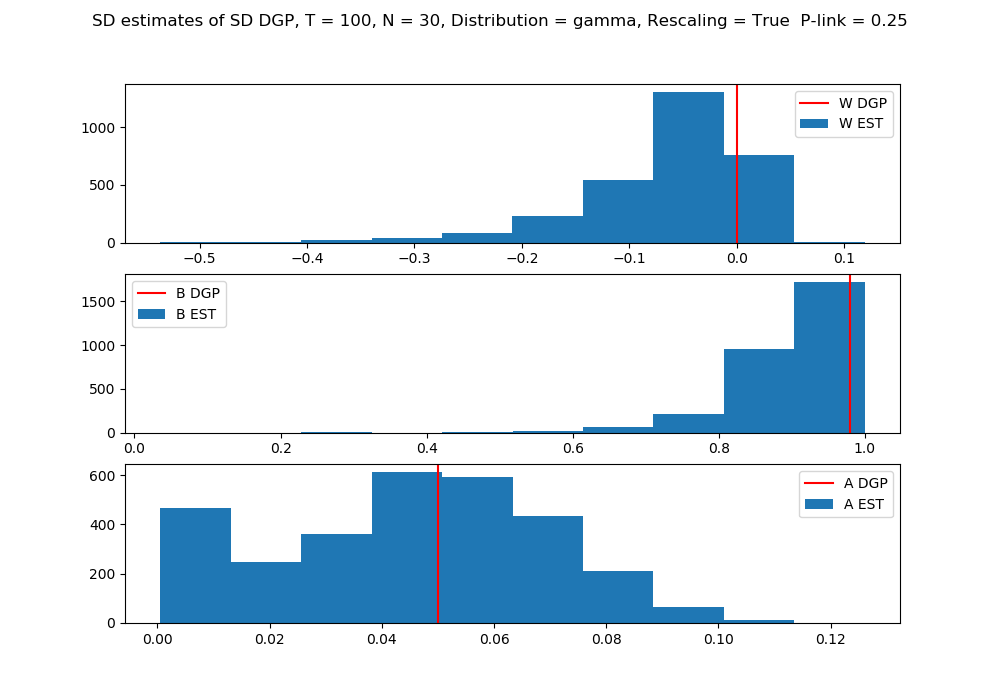
\includegraphics[width=0.95\linewidth 	]{./figures/static_SD_par_est_gamma_resc_p_0_9.png}
	\caption{Some issues with the lognormal estimate. }
\end{figure}

\subsection{Filter Misspecified Temporal Evolution} 
\begin{figure}[h]
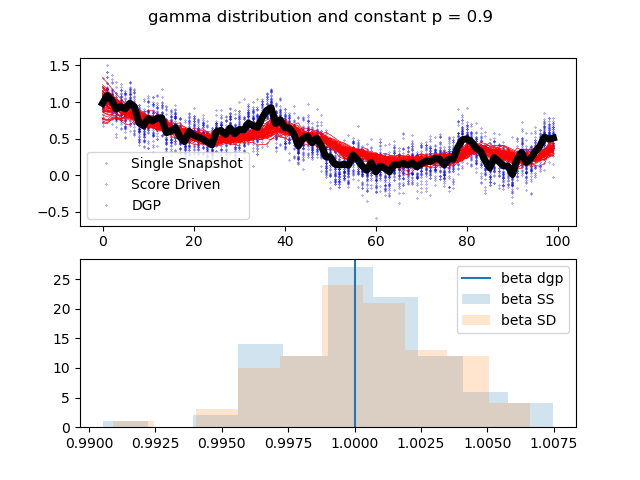
\includegraphics[width=0.45\linewidth 	]{./figures/missp_filter_ar1_gamma_no_rescale_p_0_9.png}
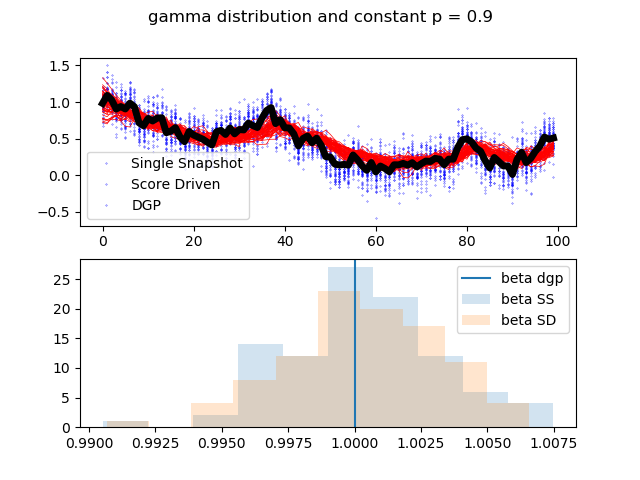
\includegraphics[width=0.45\linewidth 	]{./figures/missp_filter_ar1_gamma_rescale_p_0_9.png}\\
\caption{No rescaling left, with rescaling right. The average RMSE over 50 Simulations is 0.15, 0.133, 0.124, respectively for SS, SD-NO-RESC, SD-RESC}
\end{figure}
 

\subsection{Dynamics of the Binary Network: Score Driven Beta Model with Explanatory Variables} \label{sec:beta_model}
The weights dynamics in our approach is independent from the binary dynamics, and we can combine any sequence of $\graffe{p\et}_{t=1}^T$ with our proposed model. Nevertheless in the following we consider a specific example of binary dynamics, the Score Driven beta model, that is very much related with the one introduced in.. for the weights. We complement the model presented in (cite our paper) allowing for binary probabilities to depend on additional regressors, alongside two parameters for each node.

The definition of the static beta model reduces to assuming that the probability for the presence of each link can be written as
$$
 p_{ij}  = \frac{1}{1+ e^{ - \ibinpar_i - \obinpar_j }} 
$$
hence, with the notation used so far $\pi_{ij}  = e^{ - \ibinpar_i  - \obinpar_j }$.
With the aim of increasing the flexibility of the model we consider (propose?) a simple extension that allows the probability of observing a link to additionally depend on link specific regressors:
$$
p_{ij}  = \frac{1}{1+ e^{ - ( \ibinpar_i +  \obinpar_j + X_{ij} \beta_{ij} )}} 
$$
In this model, there are no impediments in writing the explicit dependence of the likelihood on the parameters $ \ibinpar $ and $ \obinpar$, that can be found in  \eqref{eq:beta_model}.  
we can consider the SD-beta model that allows parameters $\ibinpar$ and $\obinpar$ to follow a SD dynamics.
% We can  write the score as  
%$$
%\nabla\et\tonde{ \ibinpar\et , \obinpar\et }   = \left(\begin{array}{c}
%\frac{\partial  \log{P\tonde{\Yt |  \ibinpar\et , \obinpar\et }} }{\partial \ibinpar\et}\\
%\\
%\frac{\partial  \log{P\tonde{\Yt |  \ibinpar\et , \obinpar\et }} }{\partial \obinpar\et}
%\end{array} \right) = \left(\begin{array}{c}
%\sum_{i} Y_{i1}\et - p_{i1}\et\\
%\vdots\\
%\sum_{i} Y_{iN}\et - p_{iN}\et\\
%\\
%\sum_{i} Y_{1i}\et - p_{1i}\et\\
%\vdots\\
%\sum_{i} Y_{Ni}\et - p_{Ni}\et\\
%\end{array} \right)
%$$
%Among the possible choices, we use as scaling the diagonal matrix  $S_{ij}\et = {\delta_{ij} I_{ij}\et}^{-1/2} $, where $\boldsymbol{I\et} = {\mathbb E}[{\nabla\et {\nabla\et}^\prime}] $, i.e. we scale each element of the score by the square root of its variance.
%To clarify the notation, we mention that for the rest of this Section\footnote{This notation is indeed coherent with the one used in the rest of the paper, but we stress its meaning to avoid any confusion that might arise from the large number of parameters in the beta model. }, when we write $\theta$, without any arrow, we mean the vector that includes both $\ibinpar$ and $\obinpar$, that is $\theta = \tonde{\ibinpar^\prime,\obinpar^\prime}^\prime$.


\section{Applications}
In this section we show that our approach can be easily applied to real world networks and discuss how the flexibility that it allows can be exploited to gain new insight into their dynamics. We consider the publicly available data on international trade hence focusing on the dynamical network of bilateral trades between countries. As a second example we consider data from eMid: a section of the European (mostly Italian) interbank market.

The first aim of this applications is to use our model to "test" for the relevance of different effects in determining the dynamics of links' weights. In doing so we refer to standard approaches to model selection (refs to general model selection AIC and BIC) applied to choose among different versions of the model proposed in the previous sections. 
 
We conclude this section with a discussion of how our zero augmented dynamical model can be applied to the forecast of future links' presence and weights. We then use these methods to compare the out of sample performances of different models.
\subsection{Model Selection For Real Networks}
STATIC VS DYNAMICAL?\\
SINGLE SNAPSHOTS VS SCORE DRIVEN ? \\
REGRESSORS?\\
DISTRIBUTION CHOICE? ONLY FOR WEIGHTED\\
\subsubsection{Out of Sample Evaluation: Forecasting Sparse weighted Networks}
Once again we stress that the dynamics of links' weights is independent from that of the binary network, hence the model proposed so far can be combined with any other method for the forecast of binary networks.
Ideally we can evaluate the best performing model for link prediction in binary networks \citep[as discussed for example in][]{haghani2017systemic}, and combine it with our score driven approach for the dynamics of the weights.

For the purposes of links' forecasting and /or out of sample evaluation, we have different alternatives : 
\begin{enumerate}
	\item forecast $\Yijt$ with $E\pq{\Yijt\vert \Yijtm}$ (forecast a dense, probably always fully connected, network)
	\item given the $p\uij\et$ obtain a single network $\Aijt\tonde{p\uij\et}$ and  only for the non zero elements compute $E\pq{\Yijt\vert y>0 }$
	\footnote{Another possibility would be to use the SD update to compute $\varphi\et$ (using only observations at $t-1$),  compute the expected strengths sequence (depends on $\Aijt\tonde{p\uij\et}$) and then distribute the weights using RAS. A criterium would be needed for the extra weights. This method might allow us to take into account the fact that often banks split their weights in simple fractions (e.g. one third and two thirds  ): potremmo verificare quaòli banche nel passato mostrano propensione a divisione in frazioni ben definite e dare priorit\'a a queste nell'allocare i pesi. alloco prima i le pi\'u grandi con maggiore propensione a integer division e poi il resto.}
	\item We can repeat the previous point for each point on the ROC curve and maybe average?  what about the error for the false positive links? 
	\item repeat sample of the ZA distribution, compute one measure of forecast error each time and then average. Useful for model selection not for actual forecast.
\end{enumerate} 


\subsection{World Trade Network}
DATASET DESCRIPTION, LITERATURE REVIEW\\
\subsubsection{Weighted}
\begin{itemize}
	\item $T=56$, $T_{train} = 46$, out of sample tests on the remaining $10$ time points
	\item In smaple:
	\begin{itemize}
		\item likelihood ratios, for train sample strongly suggests models with more parameters: Single Snapshot over Score driven versions, and inclusion of regressors 
		\item AIC and BIC both suggest Score Driven models over Single Snapshot, log-normal over gamma and regressors (with more parameters) over non regressors	
	\end{itemize}
\end{itemize}
\begin{figure}[h]
	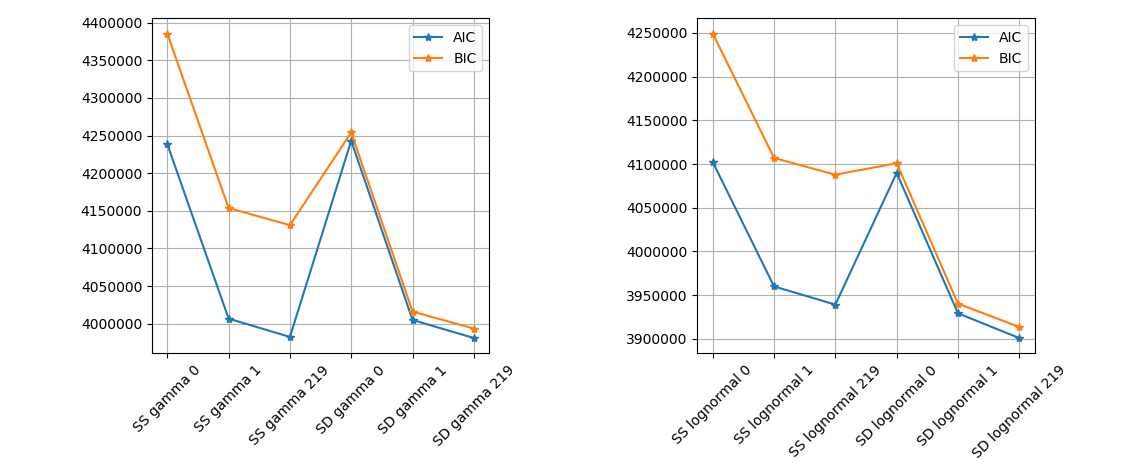
\includegraphics[width=0.95\linewidth 	]{./figures/AIC_BIC_WTN.png}\\
	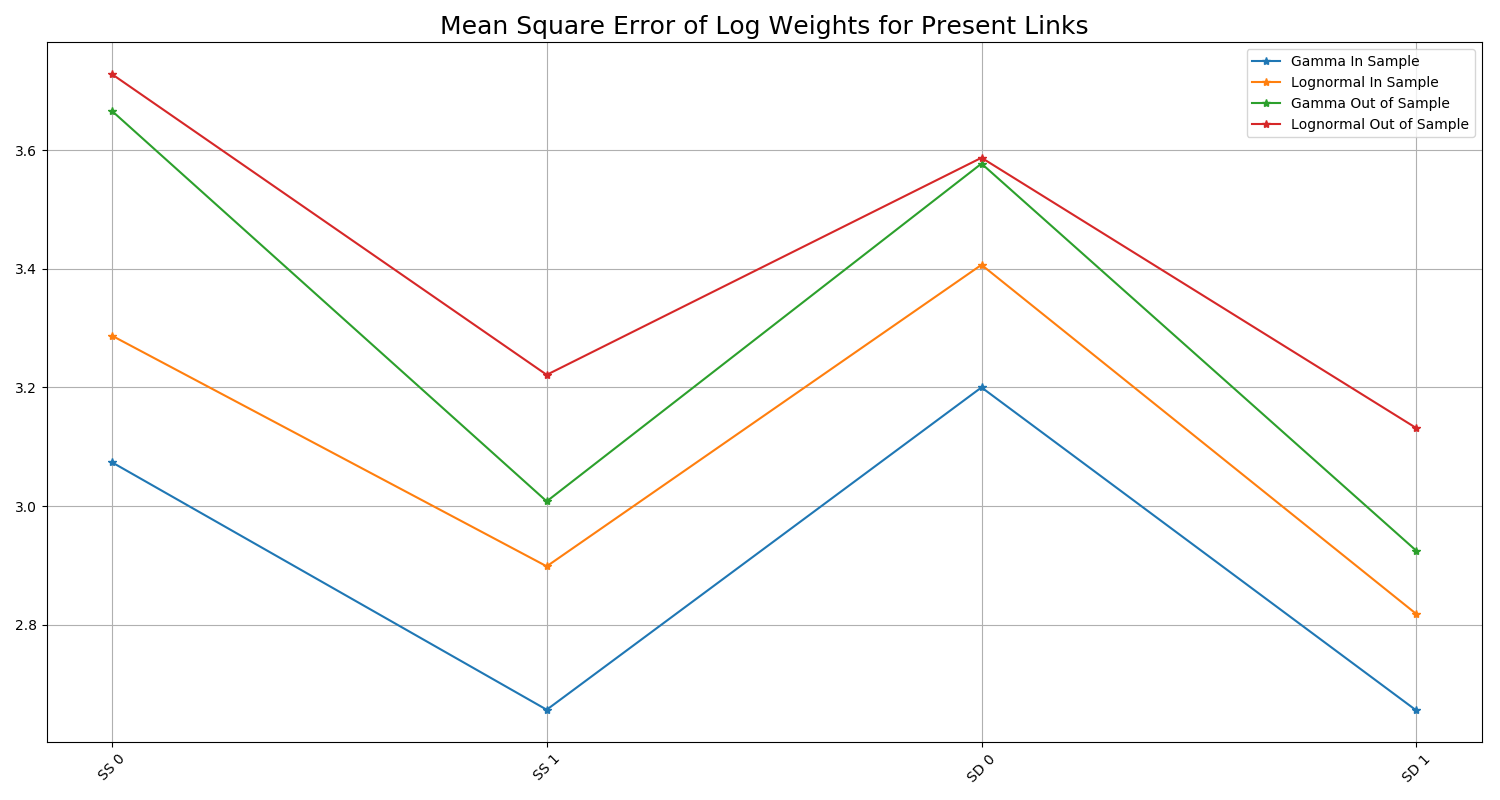
\includegraphics[width=0.95\linewidth 	]{./figures/out_of_sample_mse_log_WTN.png}\\
\end{figure}
\begin{figure}[h!]
	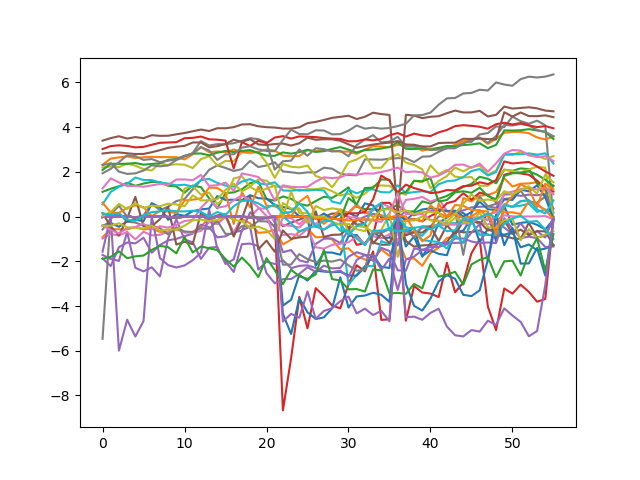
\includegraphics[width=0.95\linewidth 	]{./figures/SS_filter_WTN.png}\\
	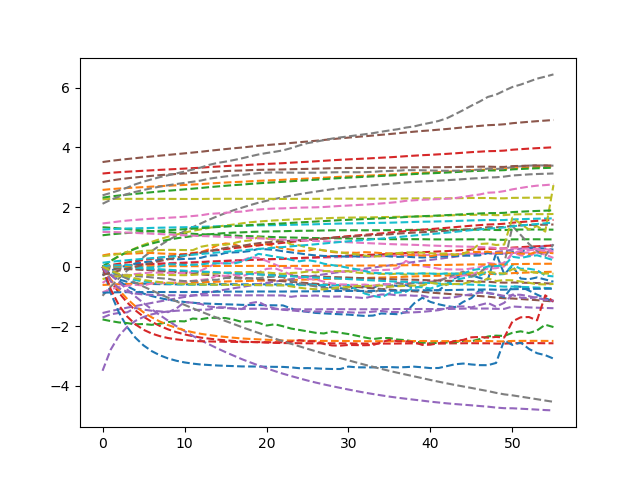
\includegraphics[width=0.95\linewidth 	]{./figures/SD_filter_WTN.png}\\
\end{figure}
\subsubsection{Binary}
\begin{figure}[h!]
	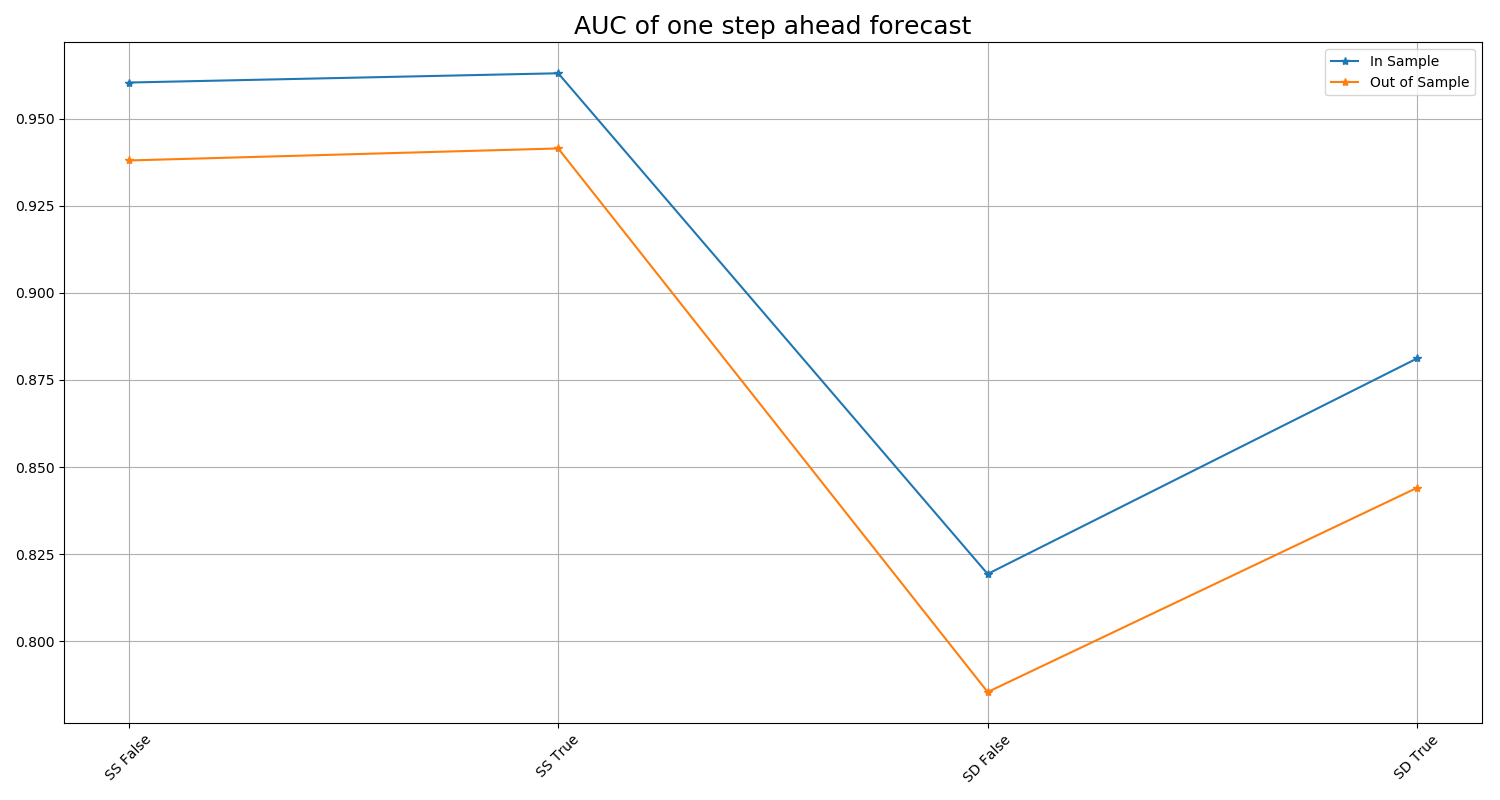
\includegraphics[width=0.95\linewidth 	]{./figures/out_of_sample_auc_WTN_bin_rescaling.png}\\
\end{figure}



\subsection{Italian Interbank Market}
DATASET DESCRIPTION, LITERATURE REVIEW\\
TEST A LINK PERSISTENCY TERM in the logit\\
TEST LIBOR EFFECT IN THE LOGIT\\
Consider also the  possibility of adding node specific regressors in the score driven update equation, e.g. the libor interest rate for eMid data 


\section{Appendix A: DynWNets, An Open Source Repository }\label{sec:appendix_code} 
The python code is available at \url{https://github.com/domenicodigangi/DynWNets}\\
A VERY BRIEF DESCRIPTION OF THE REPOSITORY AND ONE EXAMPLE SCRIPT FOLLOWED BY A DISCUSSION OF HYPERPARAMETERS TUNING AND THE USE OF PYTORCH AND BACKPROP
  
 
%\section{OLD APPUNTI Weighted Networks}
%Links' weights can be allowed to be positive integers or reals. In both cases, we need to choose what to model. 
%\begin{itemize}
%\item Given that we are interested in modeling sparse networks, we need distributions that assign a finite probability to $0$. Possibilities:
%\begin{itemize}
%\item Zero augmented distributions:
%\begin{itemize}
%\item \citep{Hautsch2014}. ZA-MEM (Zero Augmented MEM) and DZA-MEM (Dynamical). 
%\end{itemize}
%\item Censored distributions:
%\begin{itemize}
%\item Tobit \citep{sewell2015latent,giraitis2016estimating}. Censored Gaussian.
%\item Generalized Beta \citep{harvey2017modeling}. Distribution positive support, shifted and censored.
%\end{itemize}
%\end{itemize}
%\item Seems like zero augmentation allows more flexibility, since the probability to observe a zero is not directly linked to the probability of observing a particular weight. Io propendo per ZA rispetto a shifting e censoring.
%\end{itemize} 
%
%We need to choose the probability of observing a link $\Theta\tonde{\Yijt}$ and the probability to observe a specific weight $\Yijt$. Let us disregard for the moment any dependence on $\Ytm$, and consider the following extension of the fitness model for weighted networks  
%\be\label{eq:ZeroAugWeightedNets}
%P\tonde{\Yijt  = y} =  \left\lbrace\begin{array}{ll}   p\et = logit^{-1}\tonde{ \theta\et_{i} + \theta^{\tonde{t}}_{j} + \varphi^{\tonde{t}}_{i} + \varphi^{\tonde{t}}_{j} } \quad &for \quad y=0 \\
%\\
%\tonde{1 - p\et}  g\tonde{y \vert  \mu\tonde{\varphi\et_{i} , \varphi\et_{j} },\lambda\tonde{\psi\et_i, \psi\et_j}} \quad &for \quad y>0 \end{array}\right. 
%\ee
%Where the $g$ is a density function (either for continuous or discrete rvs), with mean $\mu$ and scale/dispersion parameter $\lambda$. The parameter $\varphi_i$ is intended to be related with the weights of the links formed by node $i$, $\theta_i$ with the number of links that node $i$ forms, while $\psi_i$ with the dispersion of the weights. Allowing $p\et$ to depend on $\varphi$ is intended to take into account the possibility that a link is more likely to form when the location/scale associated is larger(or the opposite) 
% 
%
%
%\subsection{Count Valued Links}
%\begin{itemize}
%\item Inizialmente ho pensato di usare GAS per rendere dinamico ERGM 
%$$
%P\tonde{\Y|\boldsymbol{\theta}} = e^{ \boldsymbol{\theta} \boldsymbol{T}\tonde{\Y} - log{\tonde{\mathcal{A}\tonde{\boldsymbol{\theta}}}} }
%$$
%\begin{itemize}
%
%
%\item  La forma di $ \boldsymbol{T}\tonde{\Y}$ definisce il dominio dei parametri. In principle, lego il parametro con dinamica GAS \'e a $\theta$ con una link function $g$ : $\theta^{\tonde{t}} = g^{-1}\tonde{f_t}$. In pratica sorgono "problemi" gia nel WCM perch\'e il dominio \'e definito per la totalit\'a dei parametri, i.e. i vincoli che ogni parametro deve rispettare dipendono dai vincoli sugli altri. 
%Se diamo dinamica GAS ai parametri "rischio"(non sono sicuro che succeda) che durante l'evoulzione si esca dal dominio. Se invece voglio restringermi al dominio con una link function, l'evoluzione non sar\'a uguale al caso unconstrained.
% 
%\item Come primo esempio, ho provato ad implementare il Weighted Configuration Model
%$$
%P\tonde{Y_{ij} = y|\boldsymbol{\theta}} =   e^{ y\tonde{\theta_i^{\tonde{t}} + \theta_j^{\tonde{t}}} }  \tonde{1-  e^{ \theta_i^{\tonde{t}} + \theta_j^{\tonde{t}} } },
%$$
% 
%\begin{itemize}
%\item assicurarsi che il prodotto $\varphi_i  \varphi_j$ rimanga in $\tonde{0,1}$, richiederebbe una link function complicata (che non mi viene in mente), oppure una riparametrizzazione di un qualche tipo (come si fa per garantire che le matrici di covarianza rimangano definite positive). Un modo semplice per risolvere \'e $\varphi_{ij} = \frac{e^{\theta_i + \theta_j}}{1 + e^{\theta_i + \theta_j} }$, ma questo non \'e pi\'u max-entr con vincolo sulle strengths, ma max-entr con vincolo sulla matrice media uguale alla matrice da Cross Entropy (sarebbe il MECAPM di \citep{di2015assessing}). 
%Quindi, usando questa riparametrizzazione non ho la stessa evoluzione che avrei usando i parametri del ERGM.
%\item Max-entr sulla sequenza delle strengts risulta nella distribuzione geometrica, che fissa un particolare valore per la dispersione (overdispersion). 
%\item Probabilmente, se vogliamo approfondire le versioni pesate discrete, conviene orientarsi su distribuzioni meno rigide come la negative binomial. In fondo la dispersione si dovrebbe poter stimare insieme ai parametri gas (come quando si stimano i gradi di libert\'a per una student con scala che segue il GAS). Potremmo considerare modelli generali di count regression che possono gestire overdispersion and excess of zero observations \citep{cameron2013regression}. 
%\end{itemize}
%\end{itemize}
%
%\end{itemize}
%\subsubsection{Zero Augmented Negative Binomial}
%If in \eqref{eq:ZeroAugWeightedNets} we consider count weights, a possibility that accommodates for over-dispersion  is the Negative Binomial 
%$$
%   P(Y = y| \sigma, \mu) \equiv   \frac{\Gamma\tonde{y+\sigma^{-1}}}{\Gamma\tonde{y+1}\Gamma\tonde{\sigma^{-1}}} \tonde{\frac{\mu}{\sigma^{-1} + \mu}}^y \tonde{\frac{\sigma^{-1}}{\sigma^{-1} + \mu}}^{\sigma^{-1}}  
%$$
%$$
%  g\tonde{\Yijt = y| e^{\psi_i +\psi_j},  \mu\et_{ij} = e^{\varphi\et_i+\varphi\et_i}}  = \frac{\Gamma\tonde{y+1/\sigma }}{\Gamma\tonde{y+1}\Gamma\tonde{1/\sigma }} \tonde{\frac{\mu\et_{ij}}{1/\sigma  + \mu\et_{ij}}}^y \tonde{\frac{1/\sigma }{1/\sigma + \mu\et_{ij}}}^{1/\sigma }  
%$$
%
%\subsection{Continuous Valued Weighted Networks}
%\begin{itemize}
%\item Nessuna novit\'a
%\end{itemize}
%\subsubsection*{Relevant Literature}
%\begin{itemize}
%\item \citep{SEWELL2016105} Prima menzione di modelli TV per reti pesate
%\item \citep{giraitis2016estimating} The weight of each link at time t follows a Tobit model, having as regressors functions the network configuration at previous time. They allow the coefficients of the Tobit regression to be time varying and estimate them with local likelihood. The authors additionally develop the asintotic theory for the local likelihood estimates proposed.  
%\item \citep{harvey2017modeling} A DCS modelling of time series of positive continuous random variables with a relevant fraction of zeros. They use a censored Generalized Error distribution and compare their proposal with a Zero inflated alternative. The dynamic of the (single??) parameter follows a DCS update.
%\item \citep{MONFORT2017348} Ho sfogliato le prime pagine. Sembra che introducano una generalizzazione della gamma distribution, considerando una mixture. Una versione della Generalized Gamma da peso finito alle zero observations. Non ho continuato a leggere perch\'e, bench\'e abbia Laplace transform semplice, la distribution \'e complicataa e contiene una serie. Non sembra adatta a modelli Score Driven .
%\item \citep{Hautsch2014} Versione Zero augmented del MEM. Considerano sia zero augmentation statica che dinamica. La versione dinamica potrebbe risultare essere l'update GAS. Non ho controllato, ma usano una struttura autoregressiva pi\'u termine Martingale difference.
%\end{itemize}
%
%
%\subsection{Applicazioni}
%Al momento ho pensato alle applicazioni solo in occasione della domanda per una internship alla BoE. Quindi per future reference riporto qui quello che avevo proposto.
%\paragraph{Dalla application:}
%Given the interest in stress testing at the bank of England, I would like to
%investigate applications of dynamic network models to forecast future network
%configurations from present data, in order to predict the emergence of systemic risk.
%This proposal is deliberately general, and not related to a specific part of the
%financial system, or channel of contagion. That is because the dynamic network
%description that I am considering is flexible and easily applicable, whenever sets of
%financial relations can be appropriately modeled as dynamic networks. Hence,
%applications are not limited to the interbank lending relations, considered for
%example in the recent Bank of England Staff Working Paper No.662(2017), by Bardoscia,
%Barucca, Brinley, and Hill. For example, they can include less investigated portions
%of the financial system, like corporate bonds markets, and the potential fire sales
%loops started from investment funds, as considered for example in the Bank of England
%Financial Stability paper No.42-July-2017, by Baranova, Coen, Lowe, Noss and
%Silvestri.
% 

 	
 

{
\bibliography{/home/domenico/Dropbox/Multi_project_files/latex_files/bibliography/bib_domenico}\bibliographystyle{chicago}

}


\end{document}
